\documentclass[10pt,twocolumn,letterpaper]{article}

\usepackage{cvpr}
\usepackage{times}
\usepackage{epsfig}
\usepackage{graphicx}
\usepackage{amsmath}
\usepackage{amssymb}
\usepackage{booktabs}
\graphicspath{{figures/}{./}}

% Include other packages here, before hyperref.

% If you comment hyperref and then uncomment it, you should delete
% egpaper.aux before re-running latex.  (Or just hit 'q' on the first latex
% run, let it finish, and you should be clear).
\usepackage[breaklinks=true,bookmarks=false]{hyperref}

\cvprfinalcopy % *** Uncomment this line for the final submission

\def\cvprPaperID{****} % *** Enter the CVPR Paper ID here
\def\httilde{\mbox{\tt\raisebox{-.5ex}{\symbol{126}}}}

% Pages are numbered in submission mode, and unnumbered in camera-ready
%\ifcvprfinal\pagestyle{empty}\fi
\setcounter{page}{1}

\begin{document}

%%%%%%%%% TITLE
\title{Retinal OCT Disease Classification Using Traditional Feature Engineering and Transfer Learning}

\author{
Bo Kang (36895385)\\
University of Southampton\\
{\tt\small bk1m25@soton.ac.uk}
\and
Abhishek Sengupta(37313266)\\
University of Southampton\\
{\tt\small as8n25@soton.ac.uk}
\and
Bohua Shen (37472208)\\
University of Southampton\\
{\tt\small bs3e25@soton.ac.uk}
}

\maketitle

%%%%%%%%% ABSTRACT
\begin{abstract}
This project investigates four-class retinal optical coherence tomography (OCT) classification, covering choroidal neovascularisation (CNV), diabetic macular oedema (DME), drusen, and normal scans. Instead of evaluating only one modelling family, we compare a traditional computer vision pipeline with a transfer-learning pipeline under the same audited data protocol. The traditional pipeline combines HOG, LBP and SIFT Bag-of-Visual-Words features with Linear SVM, RBF-SVM and Random Forest classifiers. The deep learning pipeline evaluates five ImageNet-pretrained CNNs: ResNet18, ResNet34, ResNet50, VGG16 and MobileNetV2. Model selection is based on a patient-aware validation split and uses Macro-F1 as the main metric, since the dataset is class-imbalanced. HOG with RBF-SVM is selected as the strongest traditional model, while VGG16 is selected as the strongest deep model. On the official processed test split, their Macro-F1 scores are 0.9598 and 0.9637, respectively. Because the official test split contains patient overlap with the training set, we also report a smaller patient-disjoint subset to give a more cautious estimate of robustness. Dataset link:
\href{https://www.kaggle.com/datasets/paultimothymooney/kermany2018}{Retinal OCT Images (optical coherence tomography)}
\end{abstract}

%%%%%%%%% BODY TEXT
\section{Introduction}
Retinal OCT gives cross-sectional images of retinal layers and is commonly used to support the diagnosis of retinal diseases. From a computer vision perspective, OCT classification is a useful but non-trivial task. The images are visually structured, but disease-related patterns may be subtle, and different disease categories do not necessarily have the same level of visual separability. In addition, the way a benchmark dataset is split can strongly affect the reported performance, especially when images from the same patient appear in more than one split.

This report therefore treats OCT classification as both a modelling problem and an evaluation-design problem. We compare hand-crafted visual descriptors with transfer-learning CNNs on the same processed dataset. HOG, LBP and SIFT-based Bag-of-Visual-Words features are included because they represent different assumptions about what is useful in OCT images: edge structure, local texture and local keypoint patterns. CNN-based transfer learning is also evaluated because recent studies have shown strong performance of deep models in OCT analysis~\cite{kermany2018,sunija2021,muchuchuti2023,koseoglu2023}. More recent OCT work has further explored transfer learning and transformer-style architectures~\cite{akca2024,jaimes2025}, which makes it important to compare simpler engineered features with modern pretrained networks under a controlled protocol.

\subsection{Contributions}
The main contributions of this work are fourfold. First, we build a reproducible OCT classification pipeline with dataset auditing, processed-data export and patient-aware validation splitting. Second, we compare three traditional visual representations, HOG, LBP and SIFT-BoVW, using SVM and Random Forest classifiers. Third, we benchmark five transfer-learning CNNs with the same Macro-F1 selection criterion. Fourth, we report both the official test result and a stricter patient-disjoint subset, so that the effect of patient overlap can be discussed explicitly rather than hidden behind a single test score.

\section{Dataset and Preprocessing}
\subsection{Dataset Description}
We use the Kermany retinal OCT dataset, distributed through Kaggle. The dataset contains four diagnostic categories: CNV, DME, DRUSEN and NORMAL. The raw dataset includes 84,484 images, with the official split containing 83,484 training images, 32 validation images and 968 test images. During the initial inspection, the official validation folder was found to be too small for reliable four-class model selection. With only 32 validation images, a small number of misclassified samples could change the validation score noticeably. This is especially problematic when Macro-F1 is used under class imbalance. For this reason, the official validation folder is kept only as a sanity-check split, while model selection is performed on a larger patient-aware validation split created from the official training data.

\subsection{Audit and Split Protocol}
Before training, we audited the dataset at image level. For each sample, the manifest records the file path, original split, class label, patient identifier, image identifier, image size and corrupted-file status. No corrupted image files were detected, and patient identifiers were parsed for all images. The official training set was then divided into \texttt{train\_final} and \texttt{val\_final} by patient-aware grouping. This produced 71,557 training images and 11,927 validation images, with zero patient overlap between these two splits. Compared with the official 32-image validation set, this split provides a more stable basis for model selection while still controlling patient leakage.

The audit also revealed that the official \texttt{test\_final} split contains patient overlap with the training data. This matters because OCT scans from the same patient may share anatomical features and acquisition-specific characteristics. If such images appear in both training and testing, the test performance may be over-optimistic. We therefore evaluate the selected models in two ways. The official \texttt{test\_final} split is retained as the conventional benchmark and is used only after validation-based model selection. In addition, a stricter patient-disjoint subset is created by removing test images whose patient identifiers appear in \texttt{train\_final}. This strict subset contains 201 images. It is smaller and therefore less stable statistically, but it gives a cleaner check of cross-patient robustness.

\subsection{Preprocessing and Visualisation}
All OCT images are loaded as grayscale scans and resized to $224 \times 224$. For the processed protocol, images are exported as PNG files according to manifest-defined split and class directories. This step ensures that the traditional and deep learning pipelines use the same input organisation, rather than relying directly on the original folder structure. No random augmentation is applied during validation or testing. Fig.~\ref{fig:data_distribution} shows the class distribution across the final splits. The training set is imbalanced, with CNV and NORMAL appearing more frequently than DRUSEN. This imbalance is one reason why Macro-F1 is used as the primary metric instead of accuracy alone.

\begin{figure}[t]
    \centering
    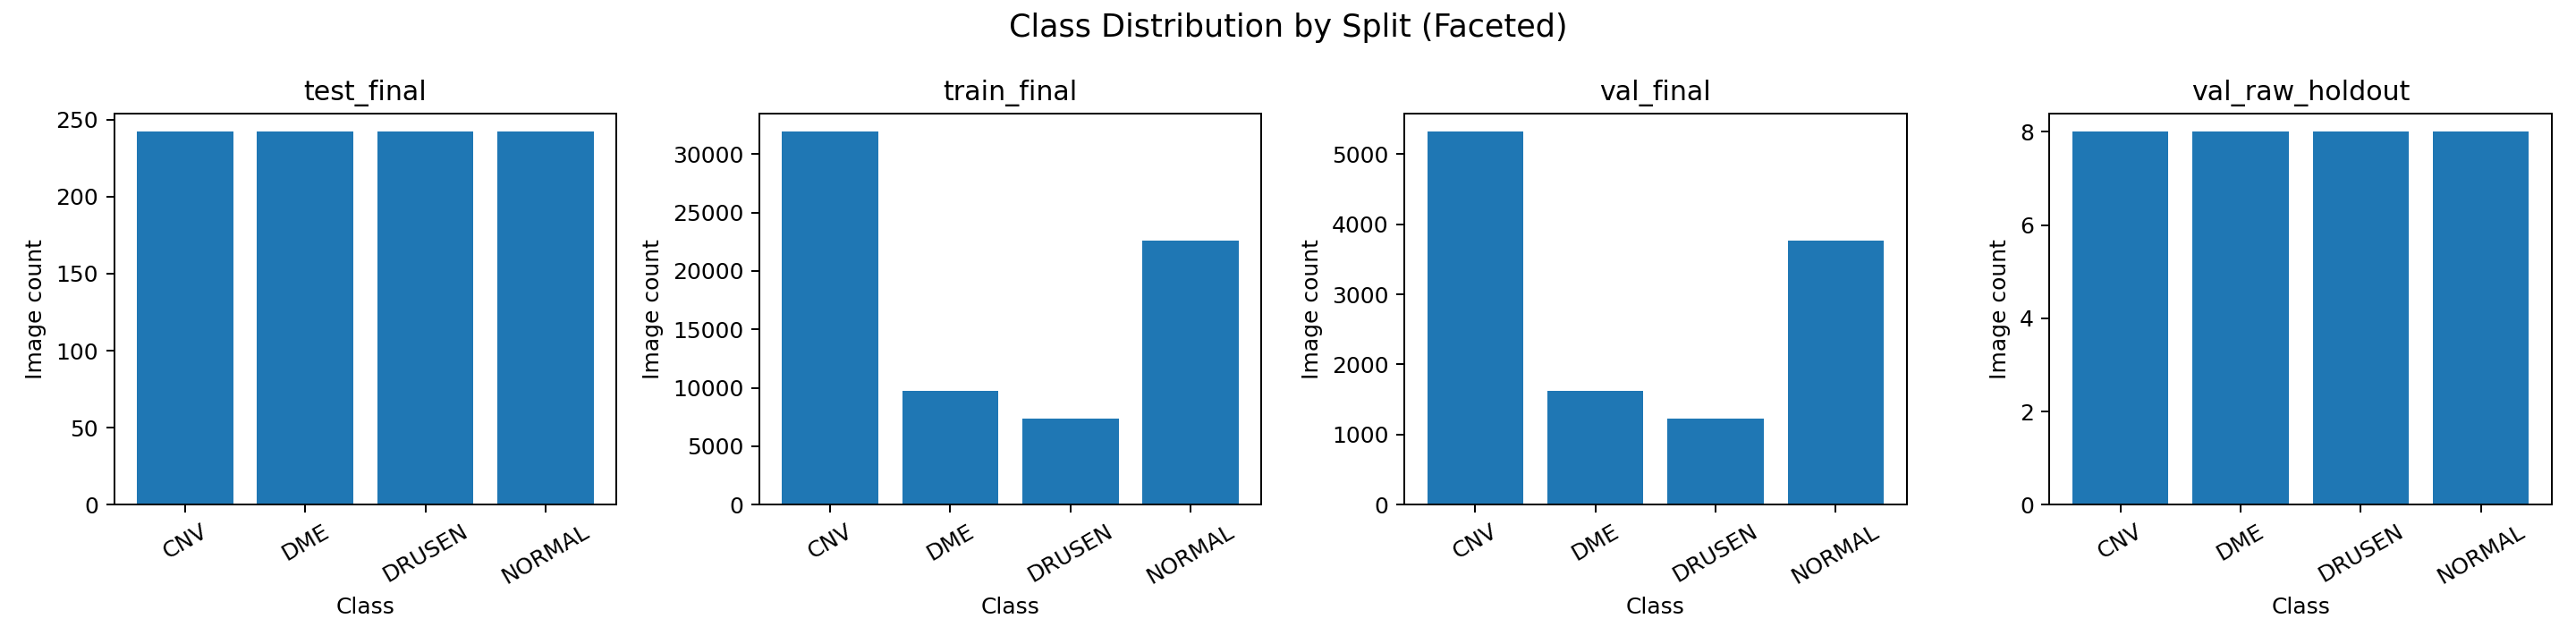
\includegraphics[width=\linewidth]{data_distribution_faceted.png}
    \caption{Class distribution across the final manifest-defined splits. The official validation folder is kept only as a sanity-check split because it contains only 32 images.}
    \label{fig:data_distribution}
\end{figure}

\section{Methodology}
\subsection{Traditional Computer Vision Pipeline}
The traditional pipeline first converts each OCT image into a fixed-length feature vector and then trains a classical classifier. We use three feature families because each captures a different type of visual evidence. HOG encodes gradient orientation histograms and is expected to represent retinal layer boundaries and lesion-related structural changes~\cite{dalal2005}. LBP captures local texture and is included because LBP-based OCT classification has been explored in retinal disease detection~\cite{yu2023}. SIFT-BoVW extracts local keypoint descriptors and pools them through a visual vocabulary, which tests whether local anatomical patterns remain useful after spatial aggregation. The HOG descriptor can be expressed as
\begin{equation}
    \mathbf{x}_{HOG}=[h_1,h_2,\ldots,h_K],
\end{equation}
and the BoVW histogram can be written as
\begin{equation}
    \mathbf{x}_{BoVW}(i)=\#\{d_j:q(d_j)=i\}.
\end{equation}

Each descriptor is evaluated with Linear SVM, RBF-SVM and Random Forest. Linear SVM gives a simple margin-based baseline. Random Forest provides a non-parametric ensemble baseline~\cite{breiman2001}. RBF-SVM is included to test whether non-linear decision boundaries are helpful in the feature space. Its kernel is defined as
\begin{equation}
    K(\mathbf{x}_i,\mathbf{x}_j)=\exp(-\gamma\|\mathbf{x}_i-\mathbf{x}_j\|^2).
\end{equation}
This produces a controlled $3 \times 3$ traditional experiment matrix rather than a single hand-picked comparison.

\subsection{Deep Learning Pipeline}
For the deep learning pipeline, we evaluate five ImageNet-pretrained CNNs: ResNet18, ResNet34, ResNet50, VGG16 and MobileNetV2. ResNet models use residual connections to make deeper representation learning more stable~\cite{he2016}. VGG16 is included as a high-capacity convolutional baseline~\cite{simonyan2015}. MobileNetV2 is included as a lightweight architecture based on inverted residual blocks~\cite{sandler2018}. All models use a four-class classification head. In this experiment, the pretrained backbone is frozen and only the classification head is trained. This setting reduces training time and lowers the risk of overfitting, although it also limits the model's ability to adapt fully to OCT-specific features.

The CNN experiments use the same input size, batch size and training length: $224 \times 224$ input images, batch size 32 and 20 epochs. The loss function is class-weighted cross-entropy,
\begin{equation}
    \mathcal{L}=-\sum_{c=1}^{C}w_c y_c\log p_c.
\end{equation}
Model selection is based on validation Macro-F1 rather than validation loss because Macro-F1 better reflects performance under class imbalance. During training, both validation loss and validation Macro-F1 are logged for every epoch. One-vs-rest ROC curves are also generated after training to compare class separability in a threshold-independent way.

\section{Experiments}
\subsection{Implementation and Metrics}
Experiments are implemented in Python using scikit-learn, scikit-image, OpenCV and PyTorch. The random seed is fixed to 42. Hyperparameter tuning and model selection use only \texttt{train\_final} and \texttt{val\_final}; the final test data are not used for model choice. Since the four classes are imbalanced, Macro-F1 is used as the main metric:
\begin{equation}
    F1_c=\frac{2P_cR_c}{P_c+R_c},\quad
    MacroF1=\frac{1}{C}\sum_{c=1}^{C}F1_c.
\end{equation}
Accuracy, macro-precision, macro-recall and confusion matrices are also reported to support the interpretation of the main results.

\subsection{Validation-Based Model Selection}
Table~\ref{tab:trad_val} summarises the strongest traditional validation results. A clear pattern appears in the comparison. HOG performs better than LBP, which suggests that gradient and layer-boundary information is more informative for this OCT task than local texture alone. The RBF-SVM also improves over the Linear SVM, indicating that the class boundaries in the HOG feature space are not purely linear. Based on the validation Macro-F1, HOG + RBF-SVM is selected as the final traditional model. This choice accepts a higher training cost in exchange for better validation performance.

\begin{table}[t]
\centering
\caption{Traditional validation performance. Best result in bold.}
\label{tab:trad_val}
\small
\setlength{\tabcolsep}{5pt}
\begin{tabular}{lcc}
\toprule
Model & Accuracy $\uparrow$ & Macro-F1 $\uparrow$ \\
\midrule
HOG + RBF-SVM & \textbf{0.8314} & \textbf{0.7414} \\
SIFT-BoVW + RBF-SVM & 0.7729 & 0.6892 \\
HOG + Linear SVM & 0.7620 & 0.6675 \\
LBP + RBF-SVM & 0.5397 & 0.4479 \\
\bottomrule
\end{tabular}
\end{table}

Table~\ref{tab:dl_val} and Fig.~\ref{fig:dl_val_curves} present the validation results for the CNN models. VGG16 is clearly separated from the other architectures, reaching the best validation Macro-F1 at epoch 8. Among the ResNet/MobileNet models, ResNet50 gives the strongest validation result, followed by MobileNetV2, ResNet34 and ResNet18. The learning curves support this ranking: VGG16 keeps a much lower validation loss and a substantially higher validation Macro-F1 throughout training. For the final test stage, VGG16 is therefore selected as the deep learning model. Its main advantage is discriminative performance, while its main drawback is computational cost compared with MobileNetV2.

\begin{table}[t]
\centering
\caption{Deep learning validation performance based on best validation Macro-F1. Best result in bold.}
\label{tab:dl_val}
\small
\setlength{\tabcolsep}{6pt}
\begin{tabular}{lcc}
\toprule
Model & Best Epoch & Macro-F1 $\uparrow$ \\
\midrule
VGG16 & 8 & \textbf{0.963} \\
ResNet50 & 19 & 0.763 \\
MobileNetV2 & 16 & 0.757 \\
ResNet34 & 12 & 0.728 \\
ResNet18 & 14 & 0.717 \\
\bottomrule
\end{tabular}
\end{table}

\begin{figure}[t]
    \centering
    \includegraphics[width=.90\linewidth]{learning_curve_all_models.png}
    \caption{Validation learning curves for all CNN models.}
    \label{fig:dl_val_curves}
\end{figure}

\begin{figure}[t]
    \centering
    \includegraphics[width=.90\linewidth]{roc_all_models_comparison.png}
    \caption{Per-class one-vs-rest ROC comparison for all CNN models.}
    \label{fig:roc_all_models}
\end{figure}

\subsection{Final Test and Robustness Results}
After validation-based selection, only HOG + RBF-SVM and VGG16 are evaluated on the final test protocols. Table~\ref{tab:final_results} reports results on both the official test split and the strict patient-disjoint subset. On the official test split, both selected models achieve high performance, with VGG16 slightly outperforming HOG + RBF-SVM. The strict subset changes the interpretation. HOG + RBF-SVM drops from 0.9598 to 0.8353 Macro-F1, which suggests that the official score is likely inflated by patient overlap. VGG16 remains strong on the strict subset, but this result should still be interpreted cautiously because the subset contains only 201 images.

\begin{table}[t]
\centering
\caption{Final test performance. Best result in bold.}
\label{tab:final_results}
\small
\setlength{\tabcolsep}{4pt}
\begin{tabular}{llcc}
\toprule
Method & Protocol & Acc. $\uparrow$ & Macro-F1 $\uparrow$ \\
\midrule
HOG+RBF & Official & 0.9597 & 0.9598 \\
HOG+RBF & Strict & 0.8557 & 0.8353 \\
VGG16 & Official & 0.9638 & 0.9637 \\
VGG16 & Strict & \textbf{0.9701} & \textbf{0.9655} \\
\bottomrule
\end{tabular}
\end{table}

Fig.~\ref{fig:roc_all_models} gives a class-level ROC comparison for all CNNs. The curves confirm the validation finding that VGG16 is the strongest deep model. It reaches near-perfect AUC values for CNV, DME, DRUSEN and NORMAL, with a macro-average AUC of 0.996. The comparison also shows that DRUSEN is the hardest category for the non-VGG16 models. Their DRUSEN AUC values are clearly lower than their CNV and NORMAL AUC values. 

Fig.~\ref{fig:interpretability} provides representative interpretability examples. For the deep learning model, Grad-CAM and Integrated Gradients focus on the central retinal deformation and fluid-related regions in a correctly classified DME case. For the traditional pipeline, the occlusion map shows sensitivity to the lesion area and retinal boundary, but the CNV image is still misclassified as DRUSEN.

\begin{figure}[t]
    \centering
    \includegraphics[width=.49\linewidth]{confusion_hog_rbf_svm_test_final.png}
    \includegraphics[width=.49\linewidth]{confusion_dl_vgg16_test_final.png}
    \caption{Confusion matrices for the selected traditional and deep learning models on the official test split.}
    \label{fig:confusion}
\end{figure}

\section{Discussion}
The results confirm the need for the revised evaluation protocol. The official validation set contains only 32 images, and the official test set has patient overlap with the training data. Therefore, models are selected on \texttt{val\_final}, while a strict patient-disjoint subset is reported as an additional robustness check. 

For the traditional pipeline, HOG + RBF-SVM is selected as the final baseline because it offers the best balance between performance and interpretability. HOG is suitable for OCT images because retinal diseases often change boundaries, fluid regions and layer shapes. In comparison, LBP mainly captures local texture, while SIFT-BoVW weakens spatial information through visual-word pooling.

For deep learning, both the learning curves and ROC results support the selection of VGG16. It achieves consistently stronger validation Macro-F1 and better class separability than the other CNNs. 

However, the VGG16 result should be interpreted cautiously. Since the backbone is frozen, the experiment mainly tests transferred ImageNet features rather than fully OCT-specific learning. In addition, the official test result may be affected by patient overlap, and the strict subset contains only 201 images. Thus, VGG16 is the strongest model within this protocol, but broader clinical generalisation still requires external patient-disjoint testing, further fine-tuning experiments and better handling of difficult classes such as DRUSEN.

\begin{figure}[t]
    \centering
    \includegraphics[width=.49\linewidth]{traditional_occlusion_example.png}
    \includegraphics[width=.49\linewidth]{dl_gradcam_ig_example.png}
    \caption{Interpretability examples for the selected traditional and deep learning models.}
    \label{fig:interpretability}
\end{figure}

\section{Conclusion}
This work compared traditional computer vision methods and transfer-learning CNNs for four-class retinal OCT classification. HOG + RBF-SVM was the strongest traditional baseline, while VGG16 achieved the best deep learning performance. The validation learning curves show that VGG16 has a clear advantage over the other CNN architectures, and the ROC analysis further confirms its stronger class separability across CNV, DME, DRUSEN and NORMAL. The study also highlights the importance of split auditing. The official test results are high, but they should be read cautiously because patient overlap may make them over-optimistic. Reporting both the official split and a patient-disjoint strict subset gives a more balanced interpretation of model performance. Future work should prioritise external patient-disjoint testing, more careful fine-tuning strategies and stronger handling of difficult classes such as DRUSEN.

\section{Individual Contribution Statement}
Bo Kang contributed to the data audit, preprocessing, patient-aware splitting, traditional feature extraction, baseline experiments, processed-data protocol, and result visualisation. Other team members contributed to deep learning experiments, evaluation visualisations, result integration, and report formatting.

\clearpage
{\small
\bibliographystyle{ieee_fullname}
\bibliography{egbib}
}

\end{document}
